% ==============================================================================
% 第 2 章：函数与程序 (Chapter 2: Functions and Programs)
% ==============================================================================

\chapter{函数与程序}
\label{sec:ch02_functions}

就程序设计而言，“算术”只占了半壁江山；另一半则是“代数”。当然，这里的“代数”与学校里讲授的代数，其联系与差异，恰如前一章的“算术”与小学算术的关系一样。具体来说，编程所需的代数概念主要包括：\term{变量}（variable）、\term{函数定义}（function definition）、\term{函数应用}（function application）以及\term{函数复合}（function composition）。本章将以生动、平易近人的方式，带你重新认识并熟练运用这些核心概念。


% ==============================================================================
% 2.1 函数
% ==============================================================================
\section{函数}
\label{sec:2.1}

程序就是函数。正如数学函数一样，程序接收输入并产生输出。但与你以往熟悉的纯数值函数不同，现代程序能够处理丰富多样的数据：数、字符串、图像、以及它们的混合组合等。不仅如此，程序通常是由现实世界中的\term{事件}（event）触发的，而程序的输出反过来又会影响现实世界。例如，电子表格软件在监听到会计敲击键盘后，会将计算好的数值填入单元格；计算机上的日历程序会在每月最后一天自动触发月度工资结算程序。最后，程序并不一定一次性消耗掉所有输入数据，它完全可以按部就班、以增量的方式逐步处理数据。

\begin{notebox}[程序与定义]
许多主流编程语言模糊了程序与数学函数之间的深刻联系，而 BSL（初学学生语言）则将这种联系置于核心显要位置。每个 BSL 程序都由若干\term{定义}（definitions）构成，其后通常跟着一个调用这些定义的表达式。BSL 中包含两类基本定义：
\begin{itemize}
  \item \term{常量定义}：形式为 \code{(define 变量 表达式)}，我们在第~1~章中已经见过；
  \item \term{函数定义}：拥有多种形态，我们在序幕中已经初试身手。
\end{itemize}
\end{notebox}

与表达式类似，BSL 中的函数定义具有严格统一的结构形式：
\begin{lstlisting}[language=BSL]
(define (FunctionName Variable ... Variable)
  Expression)
\end{lstlisting}

也就是说，定义一个函数需要：
\begin{itemize}
  \item 写下 \code{(define (}；
  \item 写下函数名称；
  \item 跟随若干个变量名（形式参数），各变量之间用空格分隔，并以 \code{)} 结尾；
  \item 写下一个作为函数体的表达式，最后闭合右括号 \code{)}。
\end{itemize}

仅此而已！下面来看几个微型示例：
\begin{lstlisting}[language=BSL]
(define (f x) 1)
(define (g x y) (+ 1 1))
(define (h x y z) (+ (* 2 2) 3))
\end{lstlisting}

在解释为什么这些例子显得“愚蠢”之前，我们先要阐明函数定义的真正内涵。粗略地说，函数定义为程序引入了一种针对数据的新运算；换言之，如果把原生操作看作语言自带的基础词汇，那么自定义函数就是向我们的词汇库中扩充了新的动词。与原生函数一样，自定义函数接收输入。\term{函数头}（header）中的变量数量决定了该函数接收多少个输入——这些输入也被称为\term{实参}（arguments）或\term{形参}（parameters）。因此，\code{f} 是单参数函数（一元函数）；\code{g} 是双参数函数（二元函数）；\code{h} 则是三参数函数（三元函数）。而紧随其后的表达式——通常被称为\term{函数体}（function body）——决定了函数计算出的返回值。

上面几个例子之所以显得“愚蠢”，是因为它们的函数体表达式完全没有用到函数头中声明的任何变量。既然变量代表输入，不在函数体中引用变量就意味着函数的返回值完全不受输入的影响，每次计算都返回千篇一律的固定常数。如果输出永远一成不变，我们根本不需要劳师动众地去编写函数或程序。

变量不是具体的数据，而是\term{代表}（represent）数据的占位符号。例如常量定义：
\begin{lstlisting}[language=BSL]
(define x 3)
\end{lstlisting}
明确表示 \code{x} 始终代表数值 3。而函数头中跟随在函数名后面的变量，则是尚未确定的未知数据的\term{占位符}（placeholder），代表着函数被调用时传入的输入数据。在函数体中引用这些变量，就是在函数被应用、实参已知时，使用这些输入数据的唯一途径。

思考下面这个尚未完成的定义片段：
\begin{lstlisting}[language=BSL]
(define (ff a) ...)
\end{lstlisting}
它的函数头是 \code{(ff a)}，意味着 \code{ff} 接收一个输入，变量 \code{a} 是该输入的占位符。在定义函数时，我们当然无法预知将来会传入什么具体数据。而定义函数的全部意义，恰恰在于我们可以多次在不同输入上重复复用同一个函数！

真正有实用价值的函数体一定会引用其参数。如果我们将 \code{ff} 补充完整：
\begin{lstlisting}[language=BSL]
(define (ff a)
  (* 10 a))
\end{lstlisting}
这就明确表达了：该函数的输出总是其输入值的 10 倍。显然，这个函数期望传入数值作为参数，因为把图像、布尔值或字符串乘以 10 是荒谬且无意义的。

现在剩下的唯一问题是：函数如何真正获取它的输入？为此，我们需要探讨\term{函数应用}（function application，即函数调用）。

\term{函数应用}是将定义好的函数投入实际运行的机制。它的语法外观与调用原生预定义操作完全一致：
\begin{itemize}
  \item 写下左括号 \code{(}；
  \item 写下自定义函数名（如 \code{f}）；
  \item 写下该函数所需数量的实参表达式，用空格分隔；
  \item 在末尾加上右括号 \code{)}。
\end{itemize}

有了这些基础，你现在就可以在交互区中尽情尝试自定义函数了。例如，下面的三组求值试验印证了前面的结论——无论传入什么输入，函数 \code{f} 产生的值永远是 1：
\begin{replbox}
> (f 1)
1
> (f "hello world")
1
> (f #true)
1
\end{replbox}

那么调用 \code{(f (circle 3 "solid" "red"))} 会返回什么呢？

\begin{notebox}[引入图像库]
若在测试中用到图像，请记得在定义区顶部添加：\code{(require 2htdp/image)}。
\end{notebox}

瞧，即使传入图像作为输入，也丝毫不会改变 \code{f} 的固定返回值。但如果传入的参数数量与函数定义不匹配，BSL 就会立即报错：
\begin{replbox}
> (f)
f: expects 1 argument, found none
> (f 1 2 3 4 5)
f: expects only 1 argument, found 5
\end{replbox}

DrRacket 发出的报错信息与原生操作参数个数不符时的报错如出一辙：
\begin{replbox}
> (+)
+: expects at least 2 arguments, found none
\end{replbox}

函数应用绝不仅限于在交互区的提示符下单独运行。我们完全可以将一个函数应用作为参数，深层嵌套在其他函数应用内部：
\begin{replbox}
> (+ (ff 3) 2)
32
> (* (ff 4) (+ (ff 3) 2))
1280
> (ff (ff 1))
100
\end{replbox}

\begin{exercise}{点到原点的距离函数}{11}
定义一个函数，接收两个数 $x$ 和 $y$，计算点 $(x,y)$ 到坐标原点的距离。

在练习~\ref{ex:1} 中，你已经针对具体的 $x$ 和 $y$ 编写了该公式的计算表达式。现在只需为该表达式配上合适的函数头。
\end{exercise}

\begin{exercise}{正方体体积与表面积}{12}
定义函数 \code{cvolume}，接收一个等边正方体的边长，计算其体积。如果你有充裕的时间，不妨顺便定义计算其表面积的函数 \code{csurface}。

\textbf{正方体计算提示：}等边正方体是一个由 6 个完全相同的正方形封闭围成的三维几何体。正方形的面积等于边长乘以自身。正方体的表面积是 6 个正方形面积的总和；其体积则是底面积乘以边长。
\end{exercise}

\begin{exercise}{提取首字符 string-first}{13}
定义函数 \code{string-first}，从一个非空字符串中提取出它的第一个 1String 字符。
\end{exercise}

\begin{exercise}{提取尾字符 string-last}{14}
定义函数 \code{string-last}，从一个非空字符串中提取出它的最后一个 1String 字符。
\end{exercise}

\begin{exercise}{定义逻辑蕴含操作符 ==>>}{15}
定义名为 \code{==>} 的函数。该函数接收两个布尔值（不妨命名为 \code{sunny} 和 \code{friday}）。若 \code{sunny} 为假或者 \code{friday} 为真，则返回 \code{\#true}。

\textbf{逻辑蕴含说明：}数理逻辑学家将这种布尔逻辑运算称为“蕴含”（implication），通常记作 $sunny \Rightarrow friday$。
\end{exercise}

\begin{exercise}{计算图像像素总数 image-area}{16}
定义函数 \code{image-area}，计算给定图像所包含的总像素数。参考练习~\ref{ex:6} 的思路。
\end{exercise}

\begin{exercise}{图像长宽形态分类 image-classify}{17}
定义函数 \code{image-classify}，接收一张图像：若高大于宽则输出 \code{"tall"}；若宽大于高则输出 \code{"wide"}；若宽高相等则输出 \code{"square"}。参考练习~\ref{ex:8} 的思路。
\end{exercise}

\begin{exercise}{字符串连字符连接 string-join}{18}
定义函数 \code{string-join}，接收两个字符串，并将它们用下划线 \code{"\_"} 连接成一个新字符串。参考练习~\ref{ex:2} 的思路。
\end{exercise}

\begin{exercise}{在指定位置插入字符 string-insert}{19}
定义函数 \code{string-insert}，接收一个字符串 \code{str} 和一个数字 \code{i}，在 \code{str} 的第 \code{i} 个位置插入 \code{"\_"}。假定 \code{i} 是介于 0 到该字符串长度之间（含边界）的有效数值。参考练习~\ref{ex:3}。深入思考一下：当 \code{str} 为空字符串 \code{""} 时，该函数应如何运转？
\end{exercise}

\begin{exercise}{删除指定位置字符 string-delete}{20}
定义函数 \code{string-delete}，接收一个字符串和一个数字 \code{i}，从字符串中删除位于第 \code{i} 个位置的字符。假定 \code{i} 介于 0（含）到字符串长度（不含）之间。参考练习~\ref{ex:4}。\code{string-delete} 能够安全处理空字符串吗？
\end{exercise}


% ==============================================================================
% 2.2 计算
% ==============================================================================
\section{计算}
\label{sec:2.2}

函数定义与函数应用形影相随、紧密协作。如果你想要系统地设计程序，就必须彻底洞悉这种协同计算的本质机制：因为你需要在脑海中清晰预演 DrRacket 是如何执行你的代码的，以便在程序出错时迅速排查根源——而编写程序时出错是不可避免的。

虽然你在初等代数课程中可能接触过类似思想，但我们希望用我们独创的精确方式进行阐释。对一个函数应用的求值严格分为三个步骤：
\begin{enumerate}
  \item DrRacket 首先计算各个实参表达式的实际值；
  \item 检查传入实参的数量与函数定义中的形参数量是否完全一致；
  \item 若完全匹配，DrRacket 会计算该函数的\term{函数体表达式}，在此过程中，\textbf{所有形参变量都会被替换为其对应的实参值}。计算得到的最终结果，就是该函数应用的值。
\end{enumerate}

这一段表述非常严谨，让我们通过具体推导演算来进行直观体会。

首先回顾对常数函数 \code{f} 的计算推导：
\begin{lstlisting}[language=BSL]
(f (+ 1 1))
== ; DrRacket 计算出实参 (+ 1 1) 的值为 2
(f 2)
== ; DrRacket 将函数体中出现的 x 全部替换为 2
1
\end{lstlisting}
最后一步看起来有些奇特，因为 \code{f} 的函数体中根本没有出现变量 \code{x}。因此，用 2 替换 \code{x} 之后函数体依旧是 1，即其本身。

再看对函数 \code{ff} 的计算过程：
\begin{lstlisting}[language=BSL]
(ff (+ 1 1))
== ; 首先求出实参的值：(+ 1 1) == 2
(ff 2)
== ; 将 ff 函数体 (* 10 a) 中的变量 a 替换为 2
(* 10 2)
== ; 依据常规算术法则计算
20
\end{lstlisting}

最美妙的是，当你将这些代数替换法则与算术运算法则结合起来时，你就拥有了准确预测任何 BSL 程序运行结果的超能力：
\begin{lstlisting}[language=BSL]
(+ (ff (+ 1 2)) 2)
== ; 实参求值：(+ 1 2) == 3
(+ (ff 3) 2)
== ; 代换：将 a 替换为 3
(+ (* 10 3) 2)
== ; 算术运算
(+ 30 2)
== 32
\end{lstlisting}

当然，我们也可以把上述计算结果复用到更大的复合运算中：
\begin{lstlisting}[language=BSL]
(* (ff 4) (+ (ff 3) 2))
== ; 实参代换
(* (* 10 4) (+ (ff 3) 2))
== ; 计算乘法
(* 40 (+ (ff 3) 2))
== ; 复用前面的推导结果
(* 40 32)
== 1280 ; 归根到底就是纯粹优美的代数推导！
\end{lstlisting}

总而言之，DrRacket 是一个运算速度极快的代数好学生：它精通所有算术定律，且极其擅长变量代换。更棒的是，DrRacket 不仅能直接给出表达式的最终答案，还能一步一步向你展示完整的演算推导轨迹！

仔细观察 DrRacket 工具栏上的按钮，其中有一个图标类似音频播放器上的“下一曲/快进”按钮。点击该按钮，就会弹出\term{单步调试器}（Stepper）窗口，你可以逐帧步进观察定义区程序的每一步求值过程。

在定义区输入 \code{ff} 的定义，并在末尾添加 \code{(ff (+ 1 1))}。然后点击【步进】（STEP）按钮，单步求值器窗口随即呈现，如图~\ref{fig:ch02_stepper} 所示。此时你可以点击前进和后退箭头，观察 DrRacket 为求出该表达式所执行的每一个微小代数步骤。你会惊喜地发现，单步求值器的演算法则与我们手动推导的步骤完全丝丝入扣。

\begin{figure}[htbp]
  \centering
  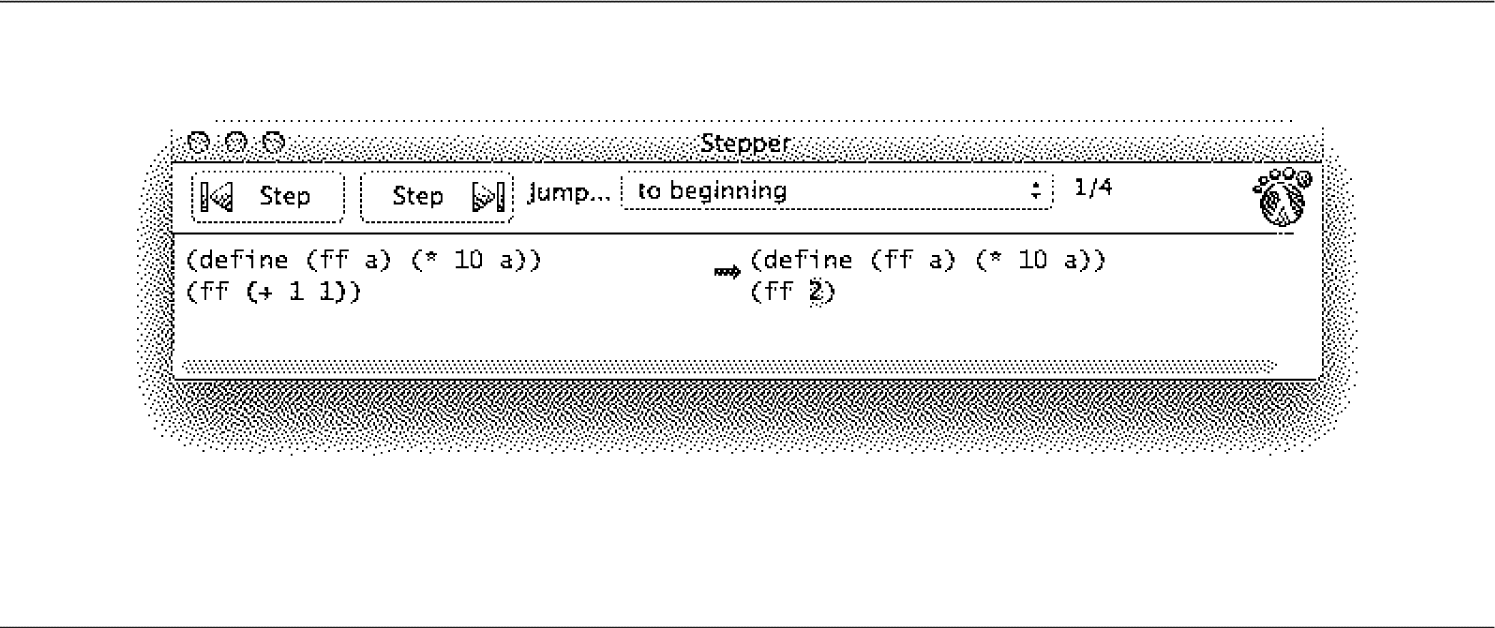
\includegraphics[width=0.75\textwidth]{images/00044.png}
  \caption{DrRacket 单步执行调试器（Stepper）}
  \label{fig:ch02_stepper}
\end{figure}

请停下来思考！是的，你完全可以用 DrRacket 来辅助检验你的代数作业。动手探索单步调试器提供的各种选项吧。

\begin{exercise}{利用单步调试器观察嵌套函数求值}{21}
在 DrRacket 中使用单步求值器逐步跟踪 \code{(ff (ff 1))} 的求值过程。然后再测试 \code{(+ (ff 1) (ff 1))}。仔细观察：DrRacket 的单步求值器会复用之前已经算好的子表达式计算结果吗？
\end{exercise}

此时此刻，你可能会觉得这与中学代数课没什么两样，尽是一些枯燥的数值与简单函数。但令人振奋的是，这一套“求值实参 $\rightarrow$ 变量代换 $\rightarrow$ 计算函数体”的计算法则，能够无缝推广到全书中所有令人惊艳的高级复杂程序！

我们来看看处理字符串的函数。回顾字符串的运算法则：
\begin{lstlisting}[language=BSL]
(string-append "hello" " " "world") == "hello world"
(string-append "bye" ", " "world")   == "bye, world"
\end{lstlisting}

现在假设我们定义一个生成信件开头的函数：
\begin{lstlisting}[language=BSL]
(define (opening first-name last-name)
  (string-append "Dear " first-name ","))
\end{lstlisting}

当给它传入两个字符串参数时，就能生成信件的称谓行：
\begin{replbox}
> (opening "Matthew" "Fisler")
"Dear Matthew,"
\end{replbox}

更为重要的是，计算法则清晰揭示了 DrRacket 是如何得出该结果的：
\begin{lstlisting}[language=BSL]
(opening "Matthew" "Fisler")
== ; 将 first-name 代换为 "Matthew"
(string-append "Dear " "Matthew" ",")
== "Dear Matthew,"
\end{lstlisting}
由于 \code{last-name} 未在函数体中被引用，用 \code{"Fisler"} 替换它不会产生任何额外影响。

本书后续章节将逐步介绍更多丰富的数据形态。而在解释各种数据上的操作时，我们始终如一地贯彻这种透明直观的代数计算法则。

\begin{notebox}[指令式操作前瞻]
在以后的高阶编程中，你可能会接触到“指令式操作”（imperative operations），它们不仅提取或组合数值，还会直接修改内存状态。要为这类操作推导演算，就需要在纯算术与代换法则之上引入额外的状态追踪机制。
\end{notebox}

\begin{exercise}{单步跟踪两点距离计算}{22}
在 DrRacket 中对以下程序片段启动单步求值器：
\begin{lstlisting}[language=BSL]
(define (distance-to-origin x y)
  (sqrt (+ (sqr x) (sqr y))))

(distance-to-origin 3 4)
\end{lstlisting}
单步求值器给出的每一步推导与你的直觉预期完全吻合吗？
\end{exercise}

\begin{exercise}{单步跟踪字符串首字符提取}{23}
字符串 \code{"hello world"} 的第一个 1String 是 \code{"h"}。下面的函数是如何计算出这一结果的？
\begin{lstlisting}[language=BSL]
(define (string-first s)
  (substring s 0 1))
\end{lstlisting}
使用单步求值器印证你的推导想法。
\end{exercise}

\begin{exercise}{单步跟踪逻辑蕴含函数求值}{24}
回顾练习~\ref{ex:15} 中逻辑蕴含函数 \code{==>} 的定义：
\begin{lstlisting}[language=BSL]
(define (==> x y)
  (or (not x) y))
\end{lstlisting}
使用单步求值器跟踪并确定表达式 \code{(==> \#true \#false)} 的一步步求值过程。
\end{exercise}

\begin{exercise}{通过单步调试修正图像分类函数}{25}
仔细研读下面这段试图解答练习~\ref{ex:17} 的初学者代码：
\begin{center}
  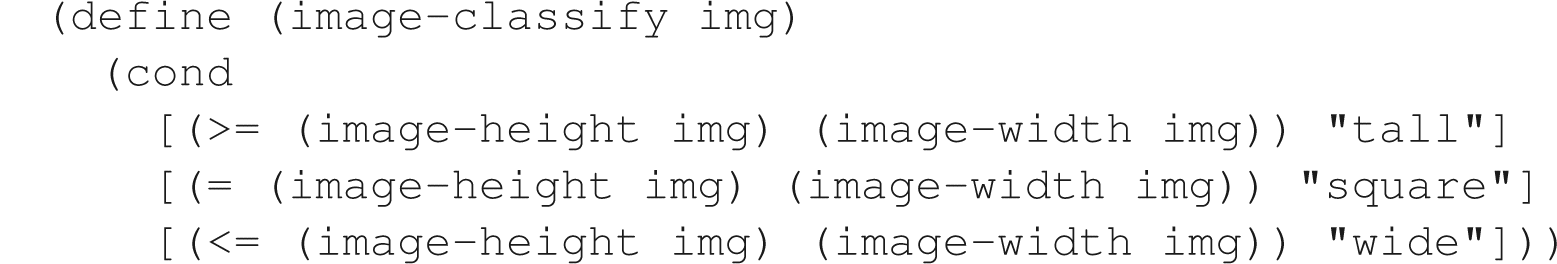
\includegraphics[width=0.8\textwidth]{images/00045.png}
\end{center}
在单步求值器中跟踪该函数在不同测试输入下的执行过程，你能发现代码中的缺陷并找到修复方案吗？
\end{exercise}

\begin{exercise}{单步跟踪复合字符串操作}{26}
在阅读并运行以下代码之前，先在脑海中预测它的执行结果：
\begin{center}
  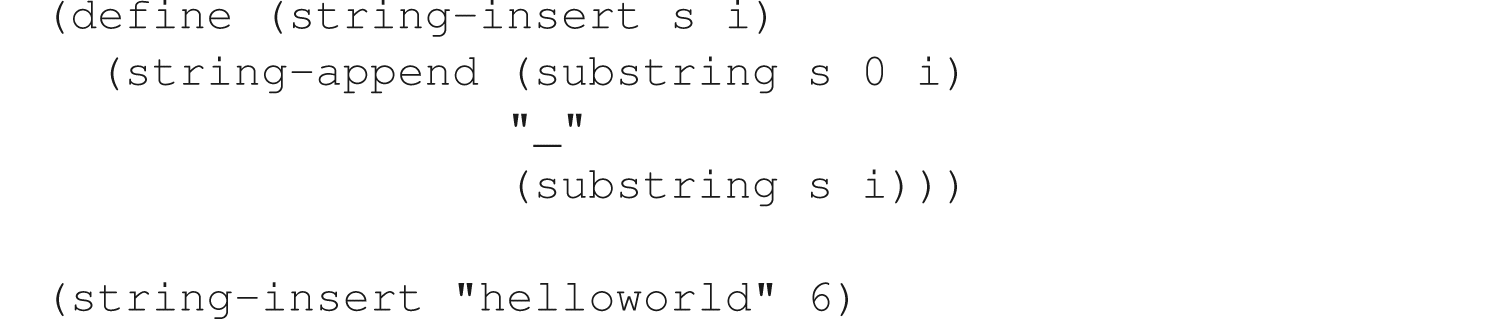
\includegraphics[width=0.7\textwidth]{images/00046.png}
\end{center}
随后在 DrRacket 中使用单步求值器验证你的预测。
\end{exercise}


% ==============================================================================
% 2.3 复合函数
% ==============================================================================
\section{复合函数}
\label{sec:2.3}

实际项目中的程序极少只由单个孤立的函数构成。典型的现代程序通常包含一个主函数和若干辅助函数，一个函数的输出往往顺畅流转为另一个函数的输入。与代数中的函数复合类比，我们将这种组织函数的方式称为\term{复合}（composition），这些协同工作的额外函数被称为\term{辅助函数}（auxiliary functions / helper functions）。

思考图~\ref{fig:ch02_batch_letter} 所示的信件模板生成程序。它由四个小函数有机协作构成：第一个是主函数 \code{letter}，它接收收件人的名、姓以及签名，生成一封完整格式的信件。主函数调用了三个辅助函数分别生成信件的三个独立部分（称谓行、正文段落和落款签名），最后通过 \code{string-append} 按正确顺序将各部分拼装合龙。

\begin{figure}[htbp]
  \centering
  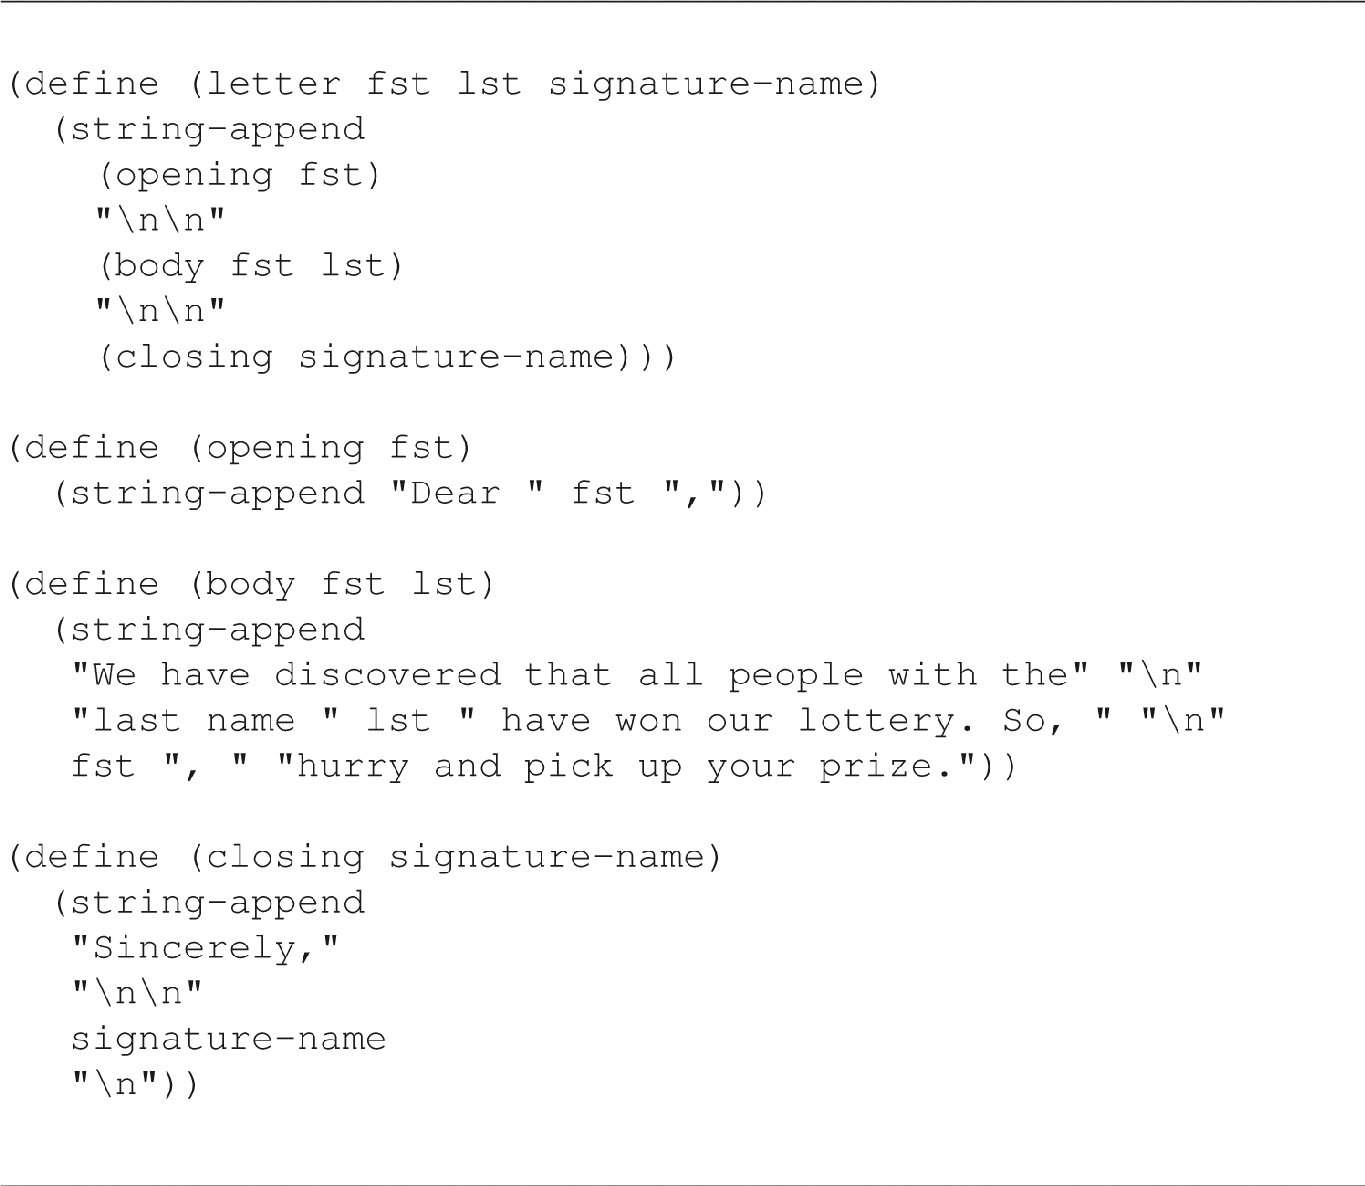
\includegraphics[width=0.85\textwidth]{images/00047.png}
  \caption{一个清晰模块化的批处理程序：信件生成器}
  \label{fig:ch02_batch_letter}
\end{figure}

请停下来思考！将上述定义输入 DrRacket 定义区，点击运行，然后在交互区中调用它们：
\begin{replbox}
> (letter "Matthew" "Fisler" "Felleisen")
"Dear Matthew,\n\nWe have discovered that ...\n"
> (letter "Kathi" "Felleisen" "Findler")
"Dear Kathi,\n\nWe have discovered that ...\n"
\end{replbox}

\begin{notebox}[控制台打印输出]
函数的返回值是一个包含换行符 \code{"\\n"} 的长字符串。如果在代码顶部加入 \code{(require 2htdp/batch-io)}，你的程序就能使用 \code{write-file} 函数，将格式化文本真实打印输出到控制台：
\begin{replbox}
> (write-file 'stdout (letter "Matt" "Fiss" "Fell"))
Dear Matt,

We have discovered that all people with the
last name Fiss have won our lottery. So,
Matt, hurry and pick up your prize.

Sincerely,
Fell
'stdout
\end{replbox}
目前可以把 \code{'stdout} 简单理解为一个代表“标准输出控制台”的特殊标记。第~2.5~节将详细剖析批处理程序。
\end{notebox}

面对一个包含多个明确计算子任务的实际问题，良好的程序架构应当贯彻黄金法则：\textbf{为每个子任务定义一个专门的函数，再由主函数统筹组装}。

\begin{notebox}[核心设计口诀]
\centering\Large\bfseries
每个任务定义一个函数\\
(Define one function per task)
\end{notebox}

遵循这一设计原则的巨大优势在于：你得到的每个小函数都足够精炼聚焦，其逻辑易于理解，它们之间的复合拓扑关系也清晰透明。一旦你掌握了科学的函数设计配方，就会深刻体会到：让一个小巧专注的函数正确工作，远比编写和调试一个庞大臃肿的巨石型函数轻松百倍！更有价值的是，当未来业务需求发生变更时，在由清晰小函数构建的模块化体系中定位并修改代码，犹如精准更换零件，比在数千行的单体代码中穿凿修改安全高效得多。

让我们通过一个经典的商业决策案例来体会这一原则的力量：

\begin{notebox}[案例研究：电影院最优票价决策]
某小镇上唯一的独家垄断电影院老板在设定电影票价时拥有完全的自主权。票价定得越高，能买得起票的观众就越少；票价定得越低，来看电影的人数就激增，但放映运营成本也随之上升。在近期的一项市场测试中，老板摸索出了票价与平均上座人数之间的精确函数关系：

当票价为每张 \$5.00 时，平均每场有 120 名观众；票价每变动 10 美分（\$0.10），平均上座人数就反向变动 15 人。也就是说，如果票价提高到 \$5.10，观众将减少到 105 人；若票价降至 \$4.90，观众将增加到 135 人。我们将这一市场规律转化为数学公式：
\[
  \text{avg.\ attendance} = 120\text{ people} - \frac{\$(\text{change in price})}{\$0.10} \cdot 15\text{ people}
\]
请停下来思考！在继续阅读之前，解释公式中减号的经济学含义。

然而，观众人数增加也会带来运营成本上升。每场放映包含 \$180 的固定运营成本，外加每位观众 \$0.04 的可变清洁服务成本。

影院老板急切想要知道：\textbf{净利润与票价之间的精确数学关系是什么？票价定在多少才能实现总利润最大化？}
\end{notebox}

虽然问题目标非常明确，但面对盘根错节的相互依赖关系，初学者往往不知从何下手。此时最佳的策略，就是贯彻口诀，将错综复杂的数量依赖关系逐一拆解为独立的纯函数：

\begin{enumerate}
  \item \textbf{上座人数依赖于票价}：计算观影人数显然是一个独立的业务规则，理应拥有专属的函数定义：
\begin{lstlisting}[language=BSL]
(define (attendees ticket-price)
  (- 120 (* (- ticket-price 5.0) (/ 15 0.1))))
\end{lstlisting}

  \item \textbf{总票房收入由售票产生}：总收入完全等于单张票价乘以观影人数：
\begin{lstlisting}[language=BSL]
(define (revenue ticket-price)
  (* ticket-price (attendees ticket-price)))
\end{lstlisting}

  \item \textbf{总放映成本由固定成本与可变成本构成}：由于观影人数本身是票价的函数，计算成本的函数同样接收票价作为参数，从而直接复用 \code{attendees} 函数：
\begin{lstlisting}[language=BSL]
(define (cost ticket-price)
  (+ 180 (* 0.04 (attendees ticket-price))))
\end{lstlisting}

  \item \textbf{最终净利润是总收入与总成本的差额}：
\begin{lstlisting}[language=BSL]
(define (profit ticket-price)
  (- (revenue ticket-price)
     (cost ticket-price)))
\end{lstlisting}
\end{enumerate}

\code{profit} 的 BSL 定义完全顺应了自然语言的问题陈述，清晰得如同一首代数诗篇！这四个各司其职的小函数共同构成了完整的利润核算程序，我们现在可以自由地在交互区中探寻最佳定价方案了。

\begin{exercise}{重构消灭魔法数：引入常量定义}{27}
我们在上面给出的示例代码中，函数体内部硬编码了许多“魔法数字”（magic numbers，例如 120、5.0、15、0.1、180、0.04 等）。正如序幕所强调的，赋予这些数字有意义的常量名称能够极大提升代码的可读性，让未来的维护者一眼看清数据来源。请将所有定义录入 DrRacket，并将所有魔法数重构为独立的全局常量定义。
\end{exercise}

\begin{exercise}{票价敏感度与影院利润最大化}{28}
使用 \code{profit} 函数分别计算票价为 \$1、\$2、\$3、\$4 和 \$5 时的潜在利润。哪一个整数票价能让影院利润最大化？在此基础上，进一步将票价精度精确到角（一角即 \$0.10），找出利润最丰厚的最佳票价。
\end{exercise}

作为对比，再看下面这个将所有计算步骤强行拼凑在单个函数体内部的“一体化单体版本”：
\begin{center}
  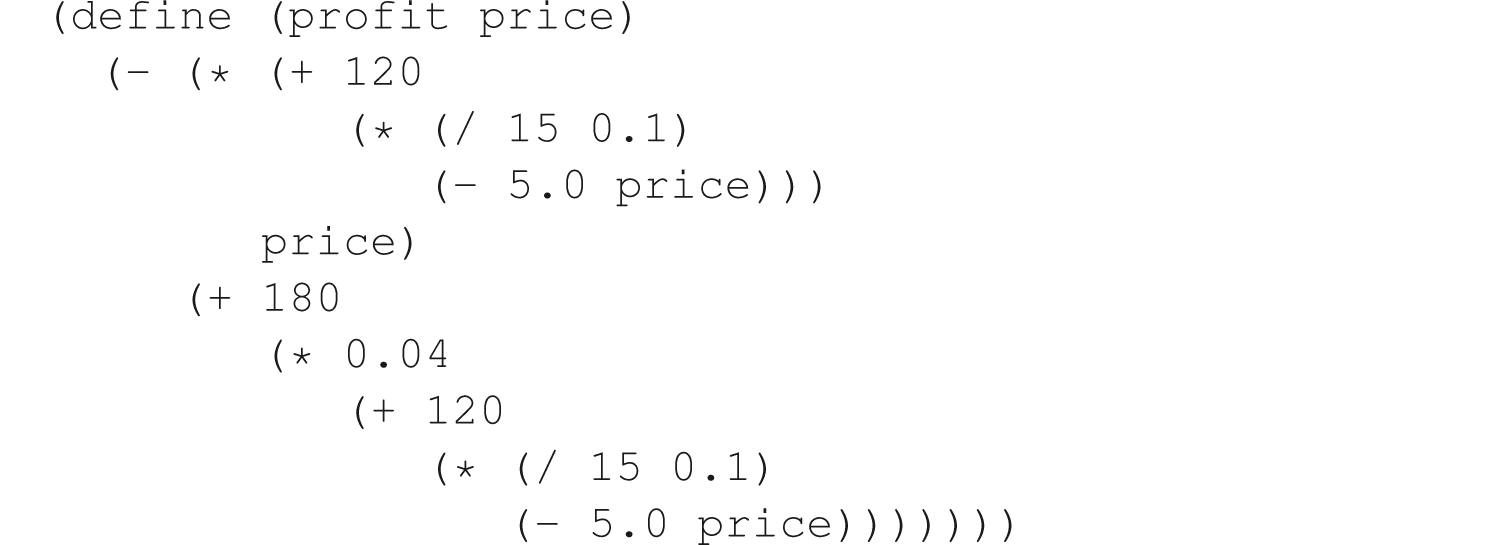
\includegraphics[width=0.85\textwidth]{images/00049.png}
\end{center}

将这个臃肿的单体函数输入 DrRacket，验证它在 \$1 到 \$5 票价下产生的结果确实与我们前面的模块化版本完全相同。但只需瞄上一眼，任何人都能立刻体会到：理解这个晦涩冗长的单体函数，比理解前面拆解明确的四个小巧函数要痛苦费力得多！

\begin{exercise}{电影院运营成本模型优化}{29}
在深入调研剧场日常开支后，老板找到了多种降低成本的有效途径。经过精益化改进后，固定放映成本被彻底削减为 0，而每位观众的可变服务成本调整为 \$1.50。

修改上述两种程序设计实现（模块化版本与单体版本）以反映这一商业规则变动。修改完成后，重新在 \$3、\$4 和 \$5 的票价下运行测试，对比两个版本的修改体验与计算结果。
\end{exercise}


% ==============================================================================
% 2.4 全局常量
% ==============================================================================
\section{全局常量}
\label{sec:2.4}

正如上文所示，类似 \code{profit} 这样的函数极大地受益于全局常量的抽取。任何完备的编程语言都允许开发者定义常量。在 BSL 中，常量定义遵循统一简洁的语法：
\begin{itemize}
  \item 写下 \code{(define}；
  \item 写下常量名称；
  \item 留出一个空格，写下一个表达式；
  \item 闭合右括号 \code{)}。
\end{itemize}

常量的名字是一个全局变量，而整条语句被称为常量定义。我们通常把常量定义中的表达式称为其“右侧表达式”（right-hand side）。

常量定义可以为任意形态的数据命名：数、图像、字符串等等。以下是一些典型示例：
\begin{lstlisting}[language=BSL]
; 当前电影票基准价格：
(define CURRENT-PRICE 5)

; 用于计算圆面积的近似圆周率：
(define ALMOST-PI 3.14)

; 换行符字符串：
(define NL "\n")

; 空白绘图背景画布：
(define MT (empty-scene 100 100))
\end{lstlisting}

前两个是数值常量，后两个分别是字符串常量和图像常量。按照工业界与函数式编程惯例，\textbf{全局常量通常采用大写字母命名}。这样可以保证无论代码库变得多么庞大，代码阅读者都能第一眼将全局常量与普通函数形参变量清晰地区分开来。

程序中的所有函数都可以自由引用这些全局变量。引用变量等同于直接使用对应的常量值。使用具名变量代替硬编码常量的最大好处在于：\textbf{一处修改，处处生效}。例如，我们想要提升圆周率的精度，或者放大画布的尺寸，只需修改一处定义：
\begin{lstlisting}[language=BSL]
(define ALMOST-PI 3.14159)
(define MT (empty-scene 200 800))
\end{lstlisting}
整个程序中所有依赖它们的地方都会自动同步更新。

我们不仅可以使用字面量来定义常量，还可以使用包含计算法则的复合表达式来定义\term{计算常量}（computed constants）：
\begin{lstlisting}[language=BSL]
(define WIDTH 100)
(define HEIGHT 200)
(define MID-WIDTH (/ WIDTH 2))
(define MID-HEIGHT (/ HEIGHT 2))
\end{lstlisting}
这里前两个常量采用字面量赋值，而后两个中心坐标常量则是通过对前两者进行代数计算得到的派生常量。

在此我们郑重提出第二条核心编程口诀：

\begin{notebox}[核心设计口诀]
\centering\Large\bfseries
问题陈述中提到的每一个常量，\\
都应为其引入一个常量定义！
\end{notebox}

\begin{exercise}{引入计算常量建模票价敏感度}{30}
为电影院最优票价程序定义一套完善的全局常量，使得“观众对票价的敏感度”（即每变动 10 美分增减 15 人）被重构为一个优雅的派生计算常量。
\end{exercise}


% ==============================================================================
% 2.5 程序
% ==============================================================================
\section{程序}
\label{sec:2.5}

现在，你已经完全具备了编写简单完整程序的全部基石！从代码构成来看，程序不过是一组函数定义与常量定义的有机集合。通常我们会明确指定一个主函数（main function），由它负责复合与调度其余辅助函数。然而从\textbf{程序启动与交互}的角度来看，软件世界主要分为两大截然不同的形态：
\begin{itemize}
  \item \term{批处理程序}（Batch Programs）：一次性接收全部输入数据，经内部管线计算后直接产出最终结果。其主函数是由辅助函数复合而成的管道。当启动批处理程序时，操作系统将输入传递给主函数，并静候其运算完成并输出。
  \item \term{交互式程序}（Interactive Programs）：以持续对话的方式运行，它消费部分输入，计算并输出部分结果，随后等待并响应新的外部输入。这种输入到达的时刻被称为\term{事件}（event），因此交互式程序本质上是\term{事件驱动程序}（event-driven programs）。这类程序的主函数通过配置明确告知操作系统：当特定类型的事件发生时，应当触发调用哪一个专属函数——这些函数被称为\term{事件处理器}（event handlers）。
\end{itemize}

当启动一个交互式程序时，主函数向宿主操作系统注册这份事件映射蓝图。每当输入事件发生，操作系统就调用匹配的事件处理器；同样，操作系统也会依据处理器的返回结果实时更新屏幕图像、播放声音等。

本书重点关注具有图形用户界面（GUI）的交互式程序；随着你继续深入探索计算机科学，你还会接触到基于网络套接字、传感器等多种形态的交互系统。

\subsection{批处理程序}

如前所述，批处理程序一次性消费所有输入数据，并由此计算出确定结果。其主函数接收参数，传递给底层辅助函数，收集各阶段的中间结果，最终整合成整体答案返回。

编写完成批处理程序后，我们可以在 DrRacket 交互区中手动调用主函数来观察其运作。而在工程实践中，更强大的用法是让程序直接从外部文件中读取数据，并将结果持久化写入新文件。历史上“批处理程序”这一称谓正源于早期计算机时代：打孔卡片被成批送入读卡机，程序读取整批卡片并在输出卡片上打孔记录结果。

通过引入 \code{2htdp/batch-io} 库，我们可以轻松构建基于文件的批处理程序：
\begin{itemize}
  \item \code{read-file}：将整个文件的文本内容一次性读取为一个字符串；
  \item \code{write-file}：接收一个目标文件名和一个字符串，将字符串完整写入该文件。
\end{itemize}

例如：
\begin{replbox}
> (write-file "sample.dat" "212")
"sample.dat"
> (read-file "sample.dat")
"212"
\end{replbox}

\begin{notebox}[文件路径安全提示]
在交互区执行读写文件命令前，请确保在 DrRacket 中先将定义区保存为一个实际的磁盘文件，以便确定相对路径基准。
\end{notebox}

执行第一句后，当前目录下会生成名为 \code{"sample.dat"} 的文件，内容为纯文本 \code{212}。\code{write-file} 返回文件名作为写入成功的确认；若文件已存在则会覆盖原有内容。第二句则把文件内容读取为字符串 \code{"212"}。

此外，\code{write-file} 还可以接收特殊符号 \code{'stdout}（标准输出设备）作为第一个参数，从而把文本直接打印在当前交互窗口中：
\begin{replbox}
> (write-file 'stdout "212\n")
212
'stdout
\end{replbox}
同理，\code{read-file} 也可以接收 \code{'stdin}（标准输入设备）从控制台交互区捕获用户键盘输入。

让我们通过一个温度换算程序来完整展示批处理程序的构建。假设我们要编写一个将华氏温度换算为摄氏温度的程序。物理换算公式如下：
\[
  C = \frac{5}{9} \cdot (f - 32)
\]
其中 $f$ 代表华氏度，$C$ 代表摄氏度。将这一公式翻译为 BSL 函数水到渠成：
\begin{lstlisting}[language=BSL]
(define (C f)
  (* 5/9 (- f 32)))
\end{lstlisting}
在交互区测试其计算精度：
\begin{replbox}
> (C 32)
0
> (C 212)
100
> (C -40)
-40
\end{replbox}

现在，我们希望将该核心算法封装进一个真正的批处理程序中：从指定文件读取华氏温度数值，进行换算，并将摄氏度结果写入输出文件。

\begin{center}
  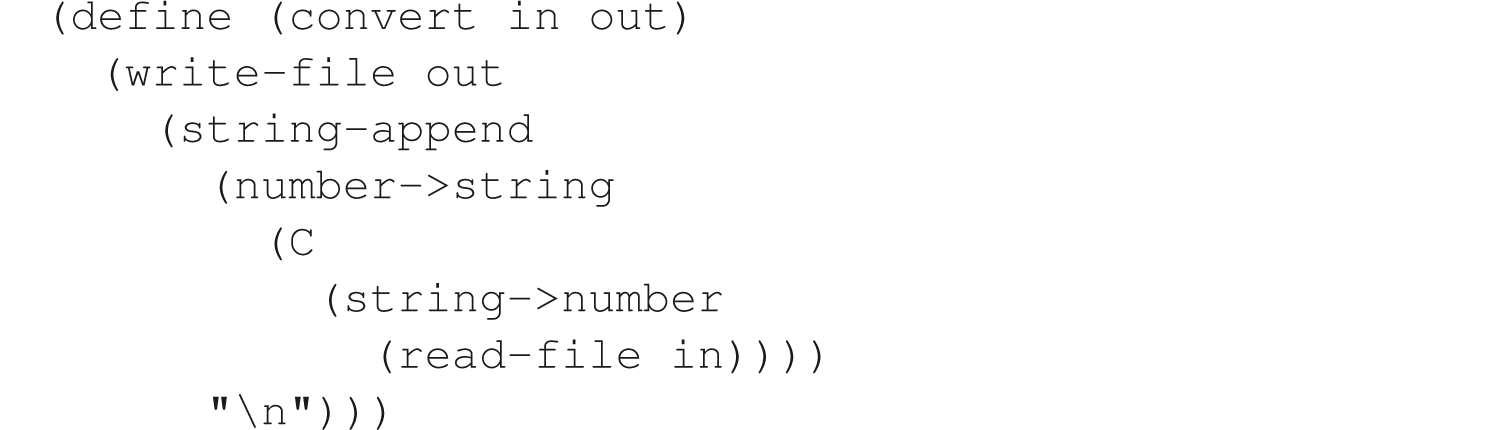
\includegraphics[width=0.85\textwidth]{images/00051.png}
\end{center}

主函数 \code{convert} 接收两个文件名参数：输入文件 \code{in} 与输出文件 \code{out}。它由 5 个函数无缝复合而成：
\begin{enumerate}
  \item \code{(read-file in)}：从输入文件读取全部内容为字符串；
  \item \code{string->number}：将该文本字符串解析为对应的数值；
  \item \code{C}：将该华氏数值精准转换为摄氏度数值；
  \item \code{number->string}：将计算出的摄氏度数值格式化为字符串；
  \item \code{(write-file out ...)}：将拼接好换行符的字符串最终落盘写入 \code{out} 文件。
\end{enumerate}

在交互区中实际测试该批处理管线：
\begin{replbox}
> (write-file "sample.dat" "212")
"sample.dat"
> (convert "sample.dat" 'stdout)
100
'stdout
> (convert "sample.dat" "out.dat")
"out.dat"
> (read-file "out.dat")
"100\n"
\end{replbox}

\begin{exercise}{运行信件生成批处理程序}{31}
回顾第~2.3~节的信件生成程序 \code{letter}。在交互区中针对至少三组不同的真实姓名调用 \code{letter} 并使用 \code{write-file} 输出到 \code{'stdout}。随后，利用下面的批处理函数，实现从三个独立文件读取姓名并生成信件文件：
\begin{center}
  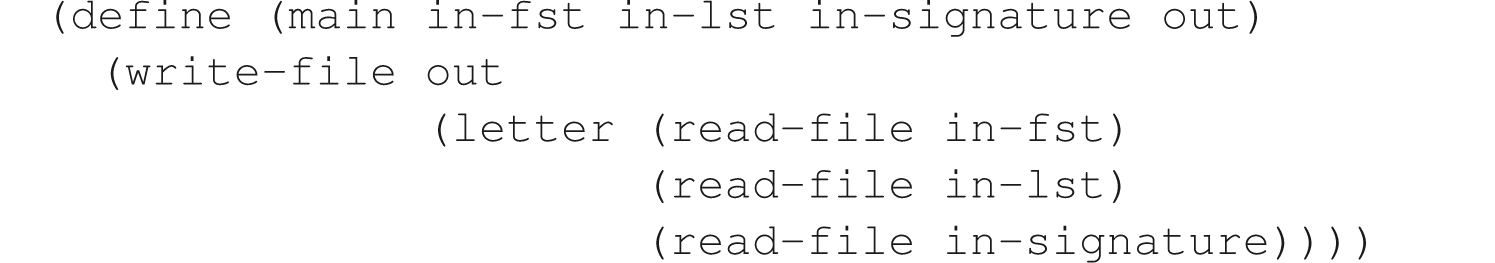
\includegraphics[width=0.85\textwidth]{images/00052.png}
\end{center}
创建输入文件，运行测试，并检查输出文件的内容。
\end{exercise}

\subsection{交互式程序}

批处理程序是商业后台计算的基石，但普通大众日常接触最多的则是图形交互软件。我们使用键盘和鼠标与桌面应用交流；此外，程序还必须时刻响应时钟跳动（clock ticks）或网络数据包到达等机器事件。

\begin{exercise}{未来交互式智能设备事件枚举}{32}
现代人不仅在台式机和笔记本上运行程序，智能手机、平板电脑和车载中控屏也已深度普及；未来更有智能眼镜、智能织物以及植入式生物芯片等新型计算形态。请列举出运行在这些前沿设备上的软件应用可能需要捕获并处理的 10 种不同形态的现实世界“事件”（events）。
\end{exercise}

孤立的计算机硬件只是一堆冰冷的物理电路。只有在安装了操作系统等系统软件后，它才具备生命力。当用户敲下键盘上的一个按键时，硬件中断会触发操作系统运行一段专门处理键盘敲击的例程。我们称这次按键为一个\term{按键事件}（key event），而处理它的函数就是\term{事件处理器}（event handler）。同理，时钟芯片每隔一定间隔发出滴答脉冲（clock tick），操作系统就执行一次时钟事件处理器。处理完毕后，系统调用渲染函数刷新显示屏像素。

面对千差万别的业务需求，不同程序需要注册不同的处理器：核电站控制程序与文字处理软件对按键的响应截然不同；火箭发射控制系统与微波炉定时软件对时钟脉冲的处理大相径庭。因此，设计一个交互式程序的核心任务，就是\textbf{向操作系统明确指定：哪一个函数负责处理键盘按键，哪一个函数负责处理时钟跳动，哪一个函数负责将程序当前状态绘制成可视图像}。

在 DrRacket 与 BSL 中，\code{2htdp/universe} 库提供的 \term{\code{big-bang}} 语法机制正是承担这一使命的指挥中枢！\code{big-bang} 负责追踪程序的当前\term{状态}（state）。它接收一个必选的初始状态表达式，以及一个必选的 \code{to-draw} 绘图子句，外加若干可选的事件监听子句。\code{to-draw} 告诉 DrRacket 如何把当前状态渲染为窗口图像；其余子句（如 \code{on-tick}、\code{on-key}、\code{on-mouse} 等）则分别指定各类事件的处理函数。

\begin{notebox}[世界程序 (World Programs) 术语]
在某种意义上，\code{big-bang} 表达式描述了程序所映射的一个微缩“世界”（World）的演进规则。这个微缩世界可能是一个贪吃蛇游戏、一个生动的物理动画，或者一个文本编辑器。因此，编程语言科学家常常将 \code{big-bang} 程序形象地称为\term{世界程序}（World Programs），并将程序的当前状态称为\term{世界状态}（State of the World）。
\end{notebox}

让我们从一个简单的绘图函数起步，逐步揭开 \code{big-bang} 的神奇面纱：
\begin{lstlisting}[language=BSL]
(define (number->square s)
  (square s "solid" "red"))
\end{lstlisting}
该函数接收一个正数，生成一个该边长的红色实心正方形。在交互区测试：
\begin{center}
  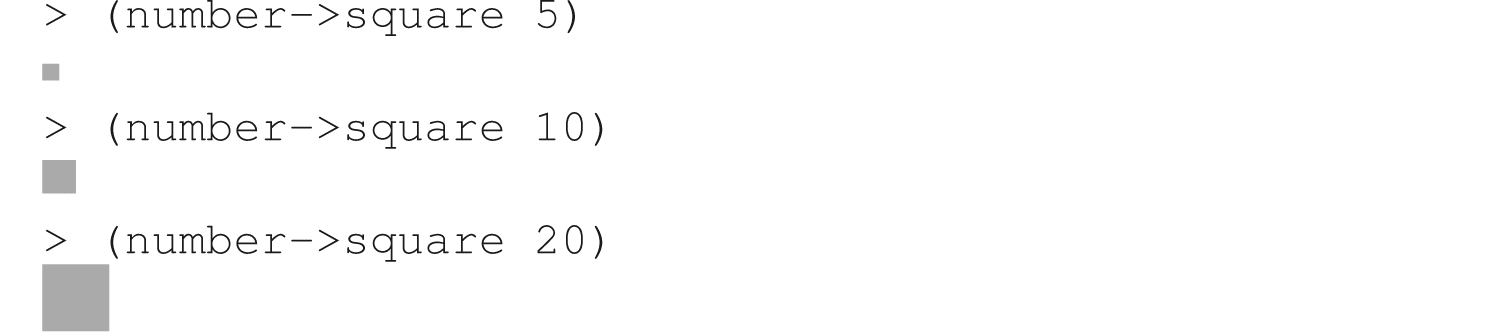
\includegraphics[width=0.7\textwidth]{images/00053.png}
\end{center}

现在在交互区输入最基础的 \code{big-bang} 表达式：
\begin{replbox}
> (big-bang 100 [to-draw number->square])
\end{replbox}

一个独立的画布窗口立即弹出，中央赫然显示出一个 $100 \times 100$ 的红色正方形！此时交互区并没有返回新的命令提示符，程序正在后台持续保持运行。点击窗口右上角的关闭按钮或 DrRacket 上的【停止】（STOP）按钮，程序终止并返回最终状态：
\begin{replbox}
100
\end{replbox}

现在看一个更加动感、功能丰富的 \code{big-bang} 表达式：
\begin{replbox}
> (big-bang 100
    [to-draw number->square]
    [on-tick sub1]
    [stop-when zero?])
\end{replbox}

这里添加了两个可选子句：\code{on-tick} 告诉系统每次时钟跳动时调用内置函数 \code{sub1}（当前值减 1）；\code{stop-when} 则指定当谓词 \code{zero?} 为真（即状态衰减到 0）时自动停止程序。整个生命周期如下：
\begin{enumerate}
  \item 初始状态为 100；
  \item 每当时钟跳动一次，当前状态减 1（经历 $100, 99, 98, \dots, 2, 1, 0$）；
  \item 每次状态发生改变，\code{to-draw} 调用 \code{number->square} 刷新窗口画面；
  \item 当状态变成 0 时，\code{stop-when} 触发，程序优雅终止并在交互区输出 0。
\end{enumerate}
你将亲眼目睹一个红色正方形在 100 个时钟周期内平滑缩小直至完全消失！

我们再进一步为它加上键盘响应能力。首先编写一个键盘事件处理函数：
\begin{lstlisting}[language=BSL]
(define (reset s ke)
  100)
\end{lstlisting}
该函数接收当前状态 \code{s} 和描述按键的字符串 \code{ke}，无条件重置返回 100。将它作为 \code{on-key} 挂载到 \code{big-bang} 中：
\begin{replbox}
> (big-bang 100
    [to-draw number->square]
    [on-tick sub1]
    [stop-when zero?]
    [on-key reset])
\end{replbox}

请停下来思考！按下回车启动程序，默数 10 秒，然后敲击键盘上的字母键 \code{"a"}，会发生什么奇妙的现象？

你会看到正方形正在一像素一像素地萎缩；然而一旦你敲下按键，\code{reset} 立即被触发并将状态重置为 100，正方形瞬间宛如充气般重新饱满膨胀到初始最大尺寸！

为了系统性地把握 \code{big-bang} 的全貌，图~\ref{fig:ch02_big_bang} 与下面的框架表达式完整展示了事件分发循环的内在逻辑：
\begin{lstlisting}[language=BSL]
(big-bang cw0
  [on-tick tock]
  [on-key ke-h]
  [on-mouse me-h]
  [to-draw render]
  [stop-when end?]
  ...)
\end{lstlisting}

\begin{figure}[htbp]
  \centering
  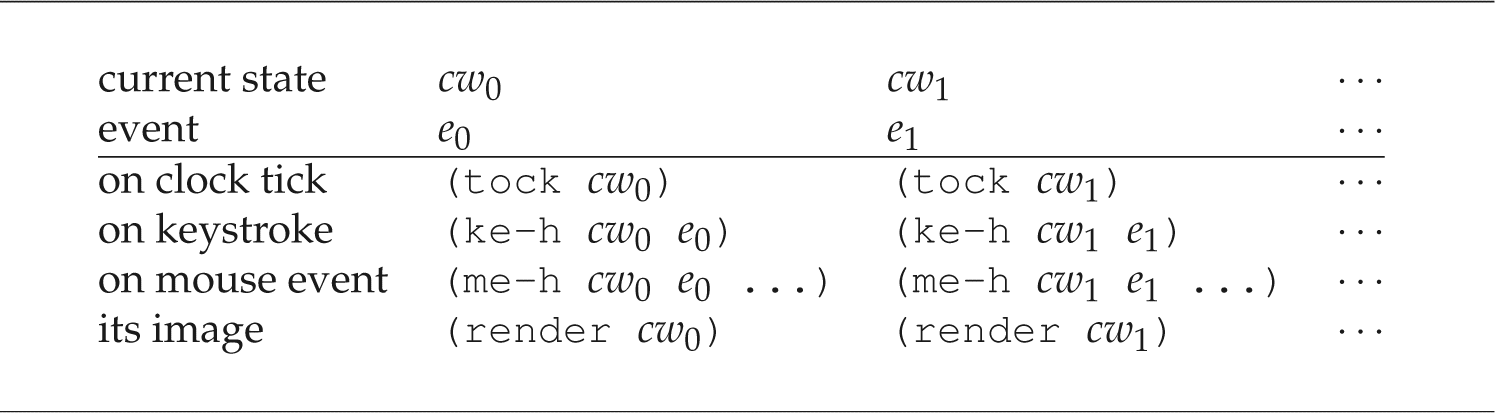
\includegraphics[width=0.95\textwidth]{images/00054.png}
  \caption{big-bang 交互式事件驱动引擎的工作机制}
  \label{fig:ch02_big_bang}
\end{figure}

事件循环的执行规则如下：
\begin{itemize}
  \item 系统以初始值 \code{cw0} 作为世界的当前状态（current world state）；
  \item 每次时钟脉冲到来，执行 \code{(tock cw)} 产出下一状态；
  \item 每次键盘敲击，执行 \code{(ke-h cw "按键名")} 产出下一状态；
  \item 每次鼠标移动或点击，执行 \code{(me-h cw x y "事件类型")} 产出下一状态；
  \item 任何事件处理完毕产生新状态后，系统首先执行 \code{(end? cw)} 检验是否应终止程序；若不终止，则调用 \code{(render cw)} 刷新屏幕图像。
\end{itemize}

图~\ref{fig:ch02_interactive_program} 给出了一个设计精巧、结构完整的第一个交互式世界程序范例：
\begin{figure}[htbp]
  \centering
  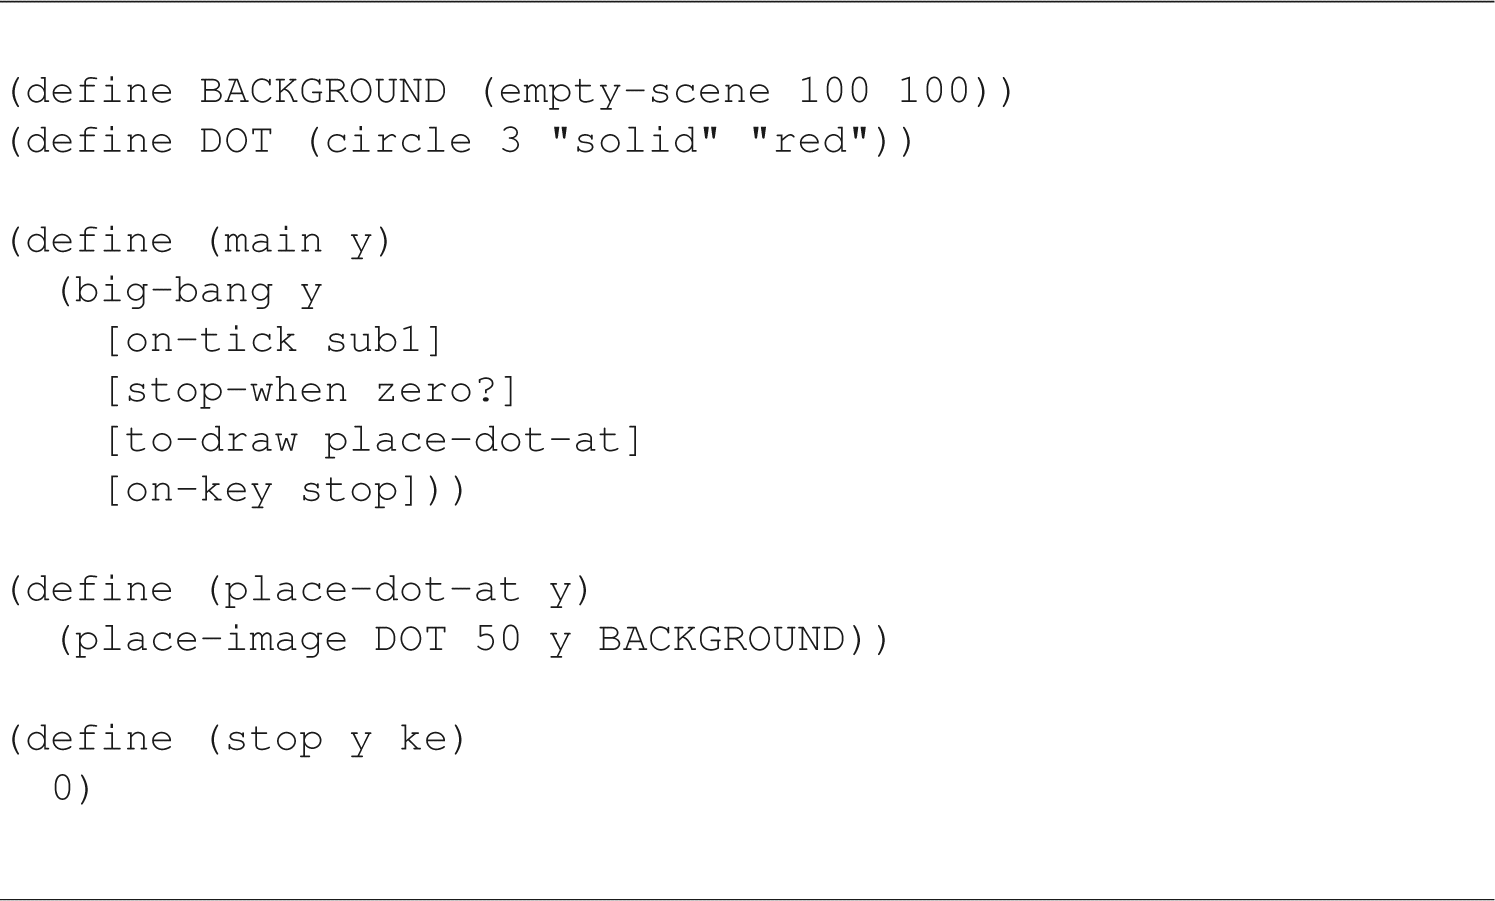
\includegraphics[width=0.85\textwidth]{images/00055.png}
  \caption{一个完整的初级交互式世界程序}
  \label{fig:ch02_interactive_program}
\end{figure}

在定义区输入该程序并点击运行，你可以在交互区中逐一调用它的各个处理函数进行独立单元验证：
\begin{center}
  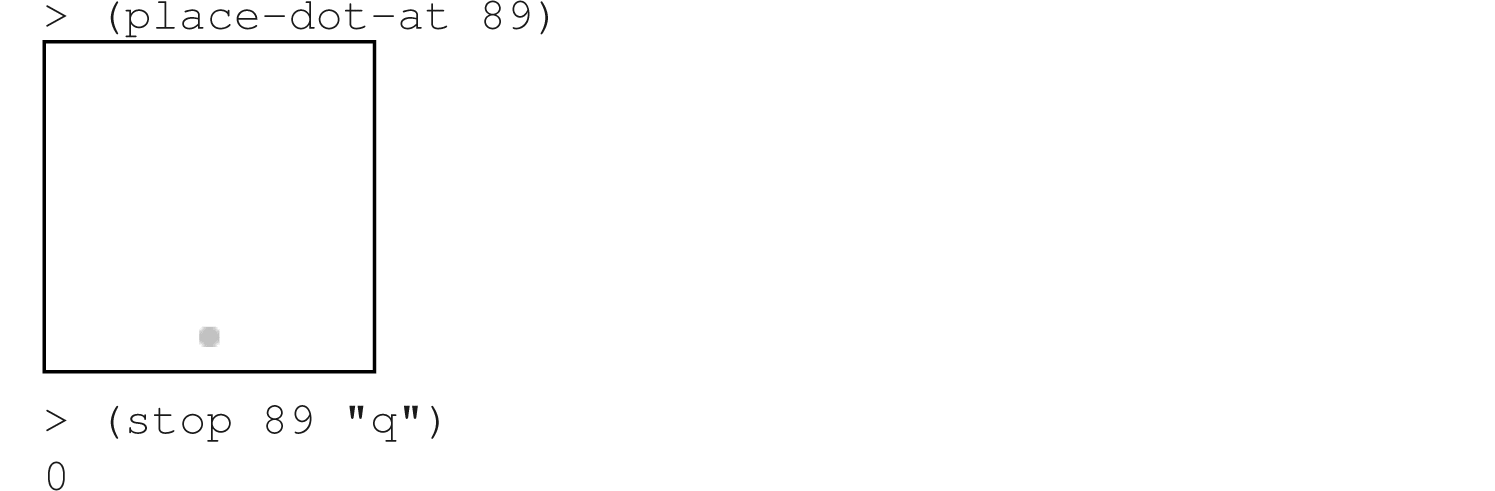
\includegraphics[width=0.75\textwidth]{images/00056.png}
\end{center}
随后调用 \code{(main 90)} 启动动画，亲手感受事件驱动编程的无穷魅力！

\vspace{1em}
\begin{notebox}[中途停歇与信心重塑]
读完前两章后，你可能会感到信息量巨大、有些应接不暇。我们学习了全新的 BSL 语言、前缀语法、求值规则、代数替换、常量规范、批处理以及基于 \code{big-bang} 的事件驱动机制。面对如此丰富的工具箱，当你拿到一个真实的问题陈述时，究竟该如何一步一个脚印地构思并设计出正确的程序呢？

别担心！下一章我们将放慢节奏，郑重为你揭晓全书的灵魂与精髓——\textbf{程序设计配方（Design Recipe）}。请稍事休息，准备迎接真正的编程思维蜕变！
\end{notebox}
